\documentclass[a4paper,11pt]{article}
\usepackage[utf8]{inputenc}
\usepackage[T1]{fontenc}
\usepackage[english,french]{babel}
\usepackage{lmodern,microtype}
\usepackage[margin=1.8cm]{geometry}
\usepackage{graphicx,booktabs,amsmath,xcolor}
\usepackage[font=small,labelfont=bf]{caption}
\usepackage[colorlinks=true,urlcolor=teal,linkcolor=black]{hyperref}
\usepackage{fancyhdr}
\usepackage[authoryear,round]{natbib}
\selectlanguage{french}
\pagestyle{fancy}
\fancyhf{}
\fancyhead[L]{\small L'autoportrait dans le rap français}
\fancyhead[R]{\small CPES DAC \textperiodcentered{} 2026--2027}
\fancyfoot[C]{\thepage}
\setlength{\headheight}{14pt}
\setlength{\parindent}{0pt}
\setlength{\parskip}{5pt}
\setlength{\emergencystretch}{2em}
\newcommand{\pct}{\,\%}
\newcommand{\rubrique}[1]{\par\medskip\textbf{#1}\par}
\hypersetup{pdftitle={L'autoportrait dans le rap français},
 pdfauthor={Agathe Salmon, Nathan Tessot, Marius Zarka et Christophe Benavent}}

\begin{document}
\thispagestyle{empty}
\begin{center}
{\LARGE\bfseries L'autoportrait dans le rap français\par}
\vspace{3pt}
{\large Aspects et transformations de l'autoportrait, 1990--2024\par}
\vspace{9pt}
{\large Agathe Salmon \quad Nathan Tessot \quad Marius Zarka\par}
\vspace{5pt}
{\small CPES Sciences des données, arts et cultures (DAC)\\
\href{https://psl.eu/formation/cpes-psl-louis-le-grand}{Université PSL et lycée Louis-le-Grand}\\
Année universitaire 2026--2027\par}
\vspace{5pt}
{\large \href{https://www.linkedin.com/in/christophebenavent/}{Christophe Benavent}\par}
{\small Université Paris Dauphine--PSL --- Dauphine Recherches en Management (DRM)\par}
\vspace{5pt}
{\small Étude exploratoire \textperiodcentered{} Résultats exportés le 28 octobre 2026}
\end{center}

{\small\textbf{Remerciements.} Les auteurs remercient ACSS-PSL pour la mise
à disposition des ressources de calcul et pour l'assistance en ingénierie
apportée à ce projet.\par}

{\small\textbf{Déclaration sur l'usage de l'intelligence artificielle.}
Selon la déclaration des auteurs, aucune rédaction directe du texte de cette
note, aucune exécution des calculs qui la fondent, ni aucune réalisation
opérationnelle du déploiement de la pile technique nécessaire à l'exécution
et à la production n'ont été effectuées par les auteurs humains : ces tâches
ont été confiées aux machines. Cette délégation ne signifie ni absence de
travail intellectuel humain ni transfert de responsabilité. Les auteurs ont
lu, pensé, conceptualisé l'étude, structuré le workflow, vérifié les résultats
intermédiaires et corrigé le processus. Ils endossent la responsabilité
du texte, des choix méthodologiques et des résultats présentés.\par}

\rubrique{Résumé}
Comment les chansons de rap français composent-elles une image de soi, et
comment les dimensions de cette image évoluent-elles entre 1990 et 2024 ?
Nous étudions un corpus stratifié de 12\,938 chansons à l'aide d'une annotation
en deux étapes par Qwen3-32B : identification des autoportraits, puis description
ordonnée de leurs aspects. Les trois résultats analysés portent sur 8\,856
descriptions valides. Le talent artistique (59,8\pct), les origines (57,6\pct)
et le caractère ou les valeurs (57,6\pct) sont les aspects les plus fréquemment
retenus. La structure des cooccurrences oppose un pôle d'affirmation
(talent, argent, rue) à un pôle introspectif (failles et émotions).
L'argent et la réussite ainsi que les failles et émotions occupent
une place plus forte dans les périodes récentes ; l'identité collective
recule. Ces résultats décrivent les annotations du corpus étudié, non une
évolution causale du genre. Leur portée reste limitée par l'échantillonnage,
l'absence de validation humaine mesurée et la fréquente saturation du nombre
d'aspects autorisé.

\textbf{Mots-clés :} rap français ; autoportrait ; humanités numériques ;
annotation automatique ; Qwen3 ; analyse diachronique.

\begin{otherlanguage}{english}
\rubrique{Abstract}
How do French rap songs construct a self-image, and how do its dimensions
change between 1990 and 2024? We examine a year-stratified corpus of 12,938
songs using a two-stage Qwen3-32B annotation workflow: self-portrait detection,
followed by ranked aspect description. The three sets of results cover 8,856 valid
descriptions. Artistic talent (59.8\%), origins (57.6\%), and character or
values (57.6\%) are the most frequently assigned aspects. Aspect co-occurrences
oppose an assertive pole (talent, money, street) to an introspective pole
(vulnerabilities and emotions). Money and success,
as well as vulnerabilities and emotions, are more prominent in recent
periods, while collective identity declines. These are descriptive patterns
in model annotations, not causal findings about the genre. Sampling,
unmeasured human agreement, and frequent saturation of the aspect limit
restrict their interpretation.

\textbf{Keywords:} French rap; self-portrait; digital humanities; automatic
annotation; Qwen3; diachronic analysis.
\end{otherlanguage}

\section{Question de recherche}
La distinction entre autoportrait et autobiographie s'appuie sur
\citet{beaujour1980}, \emph{Miroirs d'encre}. Dans notre opérationnalisation,
l'autoportrait ne se réduit pas au pronom \og je \fg{} : le locuteur assemble
les traits de sa propre image plutôt qu'il n'organise son propos autour
du récit de sa vie. Egotrip, confession et revendication de valeurs peuvent
relever de ce même geste.

\textbf{Question centrale : quelles dimensions structurent l'autoportrait
dans les chansons du corpus, lesquelles en constituent le centre, et comment
leurs fréquences évoluent-elles de 1990 à 2024 ?} Nous distinguons présence
et premier rang des aspects. L'analyse porte sur l'image énoncée, non sur
la biographie ou la sincérité des artistes.

\section{Corpus et chaîne de traitement}
\textbf{Ancrage théorique.}
La définition de l'autoportrait mobilisée dans cette étude s'appuie
principalement sur \citet{beaujour1980}, qui le distingue de l'autobiographie
par la formule : \og Je ne vous raconterai pas ce que j'ai fait : je vais
vous dire qui je suis \fg{}.
Cette distinction fonde notre attention à la composition d'une image de soi,
plutôt qu'au seul récit d'événements biographiques. L'article de
\citet{bethune2011}, \emph{Sur les traces du rap}, éclaire quant à lui
l'écriture et les outils du rappeur ; il ne constitue pas la source
principale de notre définition de l'autoportrait. La grille de douze aspects,
les prompts et les règles de décision sont une opérationnalisation propre
à cette étude, et non une grille reproduite à l'identique depuis ces travaux.

\subsection{Un échantillonnage stratifié par année}
La provenance de la base est documentée par \citet{decourson2024},
\emph{LRFAF : une exploration numérique du rap français depuis les années
1990}, disponible sur \href{https://osf.io/d96tr_v1}{SocArXiv (version 1,
publiée le 13 mars 2024)}. Ce travail constitue la référence pour la construction du corpus
à partir des paroles disponibles sur \textbf{Genius}. L'auteur décrit un
recensement d'artistes croisant Wikipédia, Wikidata et les comptes vérifiés
de Genius, puis une collecte avec LyricsGenius et un filtrage linguistique.
Le manuscrit daté du 5 février 2024 présente 37\,307 textes de 611 artistes,
diffusés dans le \href{https://huggingface.co/datasets/regicid/LRFAF}{corpus LRFAF}.
Ces effectifs sont ceux de la version décrite par l'auteur, non ceux de
notre base locale. La filiation est signalée ici, mais la révision exacte
et les opérations ayant conduit à la base locale plus étendue restent à
documenter ; nous n'assimilons donc pas les deux versions.

La base locale fournit 84\,821 chansons aux paroles exploitables après
nettoyage. Le corpus d'étude comprend toutes les 2\,438 chansons datées
d'avant 2004, puis 500 chansons par année de 2004 à 2024, tirées sans remise
avec la graine $42+\text{année}$, soit 10\,500 titres supplémentaires.
Les dates absentes, 1905 (valeur aberrante) et 2025 (année incomplète) sont
écartées. Les 12\,938 chansons couvrent ainsi 35 années. Cette construction
favorise la comparaison annuelle mais ne reproduit pas la distribution
chronologique de la base.

\begin{center}
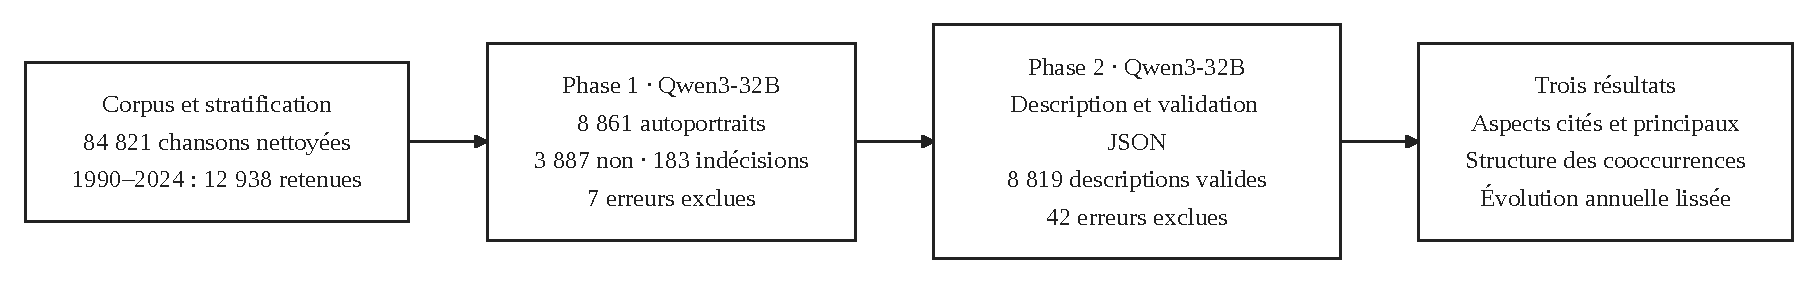
\includegraphics[width=.95\linewidth,height=6.7cm,keepaspectratio]{pipeline.pdf}
\captionof{figure}{Chaîne de traitement. Diagramme produit à partir
de la source Mermaid \texttt{pipeline.mmd}. Les erreurs techniques restent
distinctes des décisions interprétatives.}
\label{fig:pipeline}
\end{center}

\subsection{Deux étapes d'annotation, un même modèle}
La première étape applique les catégories \texttt{autoportrait},
\texttt{pas\_autoportrait} et \texttt{je\_ne\_sais\_pas}. Les exports comptent
respectivement 8\,861, 3\,887 et 183 décisions, plus 7 erreurs techniques.
Les autoportraits représentent 68,5\pct{} des chansons sélectionnées :
c'est une proportion brute de l'échantillon, non une estimation pondérée de
l'ensemble du rap français. La seconde étape ne traite que les 8\,861
autoportraits : 8\,856 descriptions sont exploitables et 5 sont en erreur.
Le suffixe \texttt{8861} des fichiers désigne donc le lot soumis,
\emph{pas} le dénominateur des graphiques.

Les notebooks utilisent \texttt{Qwen/Qwen3-32B}, servi localement par deux
instances vLLM indépendantes, une par GPU. Le raisonnement est activé ; la
température vaut 0 et le budget de sortie 8\,192 jetons, raisonnement compris.
Douze requêtes par serveur, soit 24 au total, sont distribuées par une file
de créneaux ; les lots de 128 limitent les tâches soumises. Les journaux
permettent une reprise et le client valide le JSON, les catégories et
l'unicité des listes. Ces contrôles garantissent une structure exploitable,
pas la justesse sémantique de l'annotation.

\subsection{Environnement technique et assistance au développement}
Le traitement s'appuie sur le \textbf{cluster ACSS-PSL} et ses ressources GPU.
La pile comprend \textbf{Python et les notebooks Jupyter}, pandas pour les
tableaux, Matplotlib pour les graphiques et tqdm pour le suivi des traitements.
\textbf{vLLM} expose une API compatible OpenAI pour l'inférence locale de
\textbf{Qwen3-32B} ; cette compatibilité ne signifie pas que les paroles sont
envoyées à un service OpenAI. Les échanges et exports reposent sur JSON,
JSONL et CSV.

\textbf{Claude et GitHub Copilot} ont été mobilisés comme assistants dans
l'élaboration du projet et le travail de développement. Ils doivent être
distingués du modèle d'annotation : les décisions analysées ici proviennent
de Qwen3-32B, et non d'un vote entre ces outils. Leur intervention ne constitue
pas une validation indépendante des catégories. Le versionnement repose sur
\textbf{Git et GitHub} ; le présent article utilise \textbf{LaTeX et BibTeX},
un diagramme \textbf{Mermaid} et une compilation par \textbf{Tectonic}.
Les versions exactes des assistants, des bibliothèques et du matériel de la
campagne ne sont pas établies ici ; elles ne sont donc pas déduites de
l'environnement actuel.

\subsection{Consignes : de la définition au codage des facettes}
Les prompts traduisent la distinction de \citet{beaujour1980} entre
autoportrait et autobiographie en décisions explicites, tandis que
\citet{bethune2011} nourrit la réflexion sur l'écriture et les outils du
rappeur. La grille exacte de codage reste une construction propre au projet.

\textbf{Phase 1 : reconnaître le geste d'autoportrait.}
La consigne articule deux conditions : le locuteur est le sujet du texte
(\textsc{auto}) et il compose son image plutôt qu'il ne déroule un récit
(\textsc{portrait}). Ni le pronom \og je \fg{}, ni la sincérité supposée,
ni le ton ne suffisent à décider. Le prompt distingue les portraits d'autrui,
les récits, les adresses et les ambiances ; il explicite les cas limites
(parcours de vie, engagement, amour, rivalités, collectif). La réponse doit
contenir une justification sans citation des paroles et l'une des trois
étiquettes, dont une indécision réservée aux cas réellement partagés.

\textbf{Phase 2 : décrire et hiérarchiser les facettes.}
La consigne décrit le registre (egotrip, introspection, manifeste, mixte),
un à sept aspects ordonnés parmi douze, la temporalité, les figures de
démarcation et le regard explicite d'autrui. Dans sa version actuelle,
un aspect secondaire doit être central et être le sujet principal d'un
couplet ou du refrain, ou être développé dans environ un quart du texte ;
les listes de quatre à sept aspects doivent rester exceptionnelles.
Le plafond actuel de sept remplace celui de quatre utilisé pour les
résultats présentés ici, sans modifier rétroactivement ces annotations.
La démarcation n'est pas assimilée au regard d'autrui : ce dernier exige
un jugement rapporté qui vise le locuteur.

Les deux prompts imposent de juger la chanson entière, de ne compter un
refrain répété qu'une fois et d'ignorer les connaissances externes sur
l'artiste. La réponse finale est un objet JSON à champs imposés.
Les annexes~\ref{ann:phase1} et~\ref{ann:phase2} reproduisent intégralement
les consignes textuelles actuellement présentes dans le dépôt, et non les
paroles soumises, les schémas JSON ou l'enveloppe technique des requêtes.
Faute de vérification des empreintes historiques, elles ne certifient pas
la version exacte utilisée pour produire les résultats présentés.

\subsection{Aspects et indicateurs}
La description comprend le registre, la temporalité, les démarcations, le
regard d'autrui et une liste ordonnée de un à quatre aspects parmi douze.
Nous analysons seulement cette dernière liste. Un aspect est dit
\emph{cité} s'il y figure ; il est \emph{principal} s'il arrive en tête.
\og Cité \fg{} désigne ici une catégorie attribuée par le modèle, pas le comptage
d'un mot ni une citation littérale. Plusieurs aspects pouvant être retenus,
les pourcentages de présence ne s'additionnent pas à 100\pct.

\section{Résultat 1 : les composantes de l'image de soi}
\begin{figure}[t]
\centering
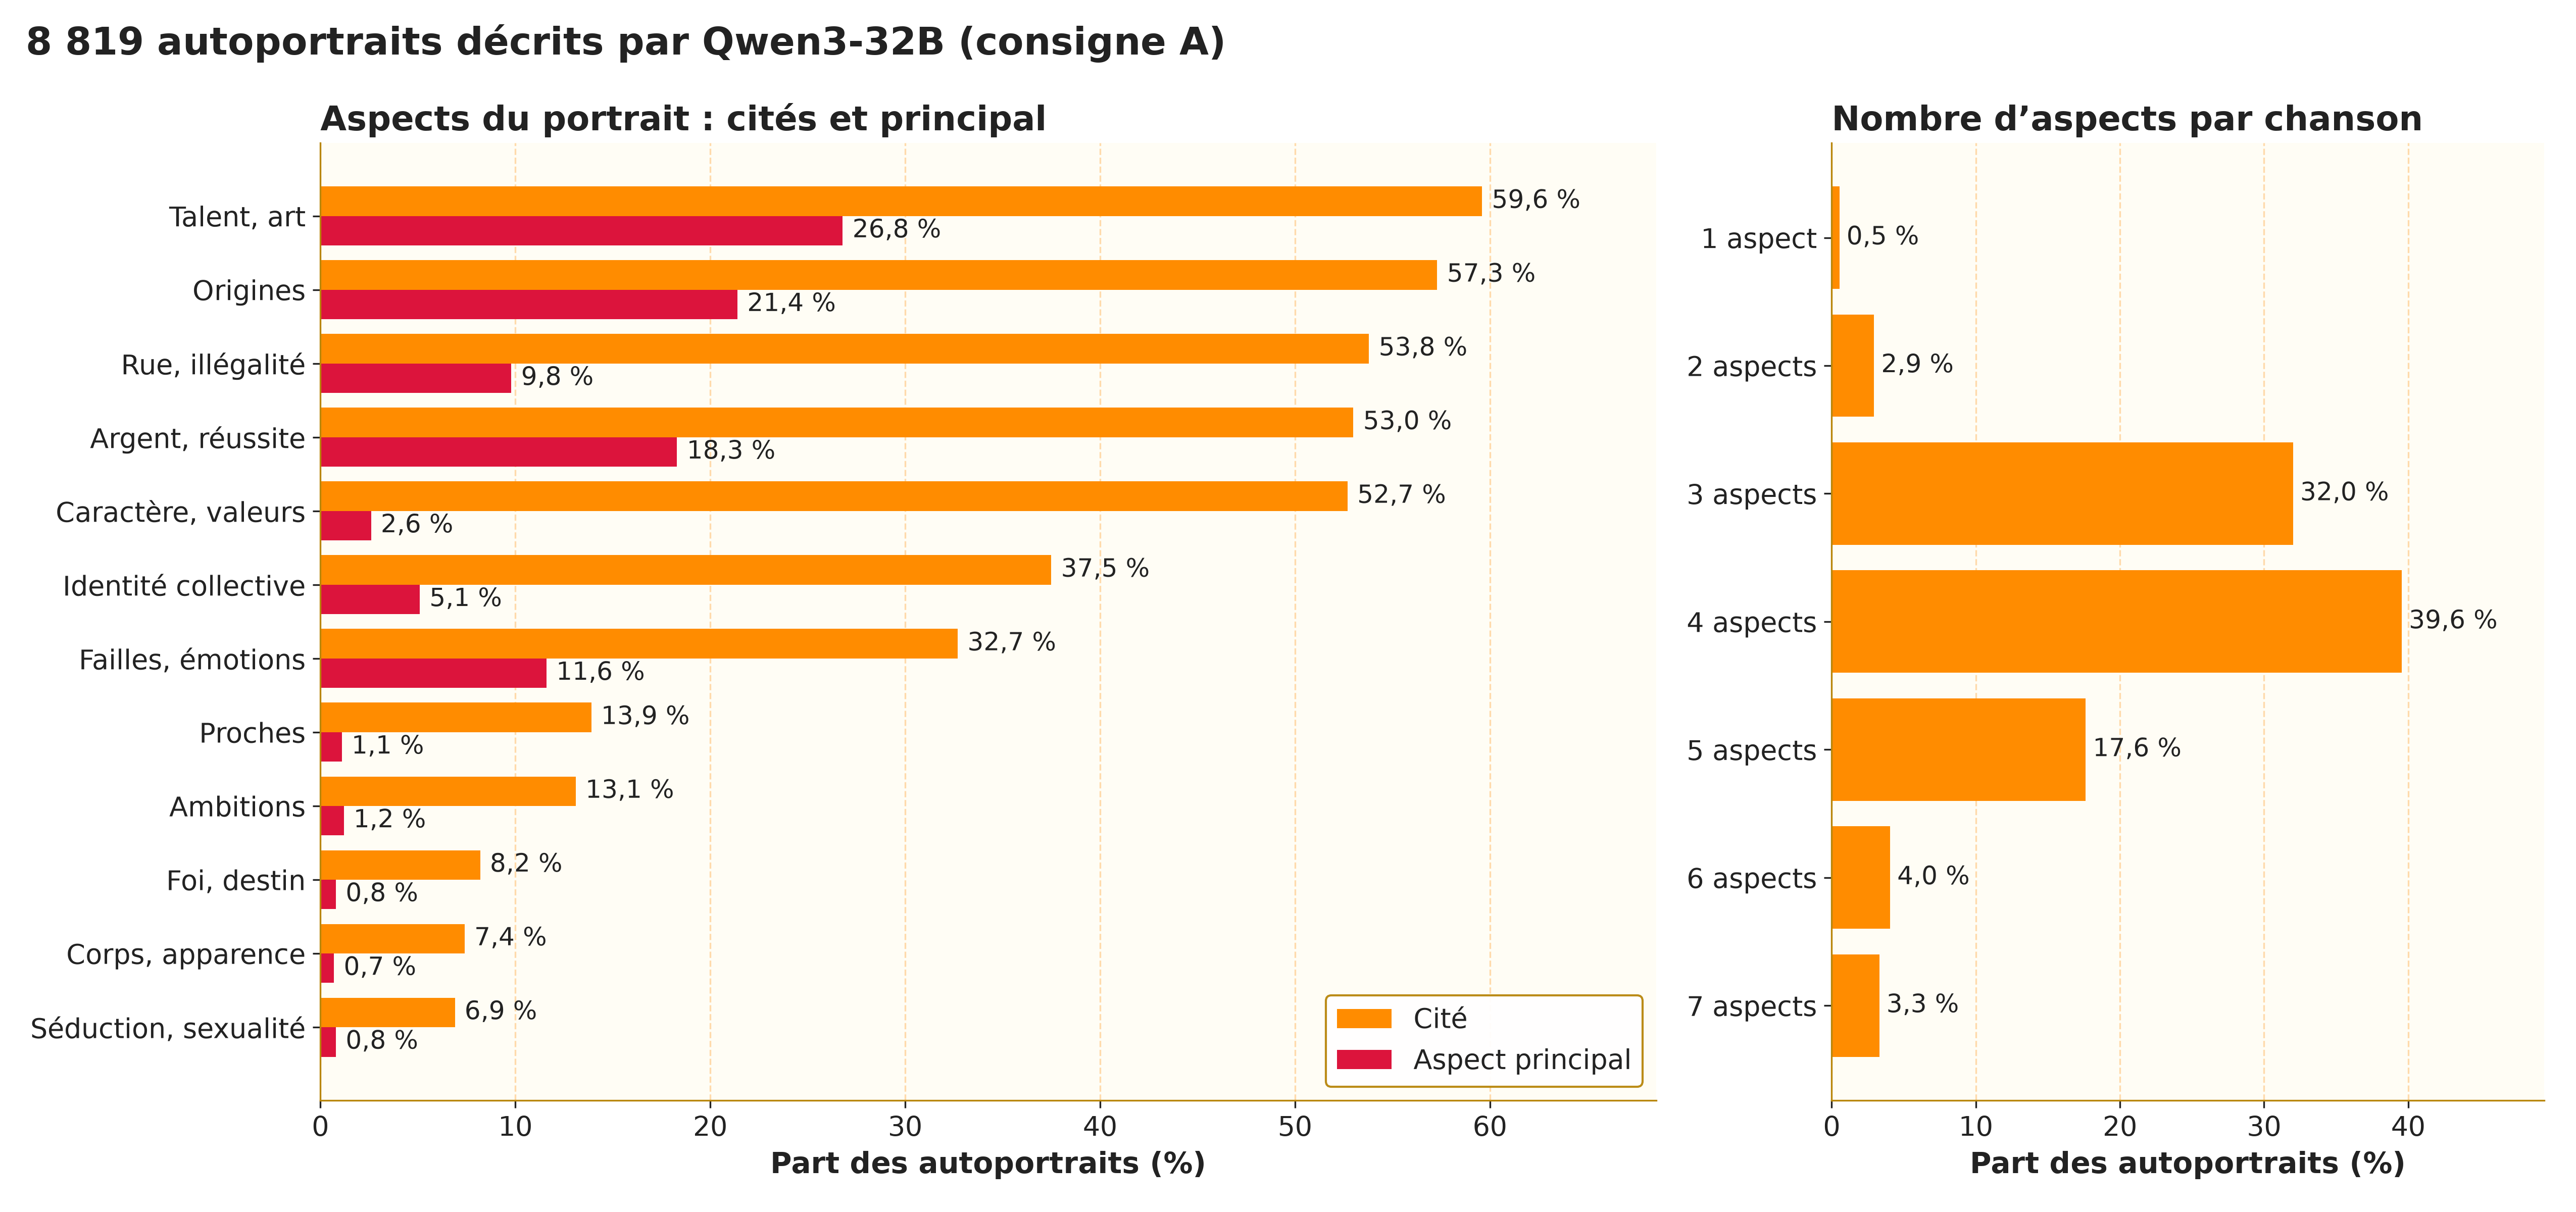
\includegraphics[width=\linewidth]{../images/autoportrait2_aspects_8861.png}
\caption{Aspects cités et principaux dans les 8\,856 descriptions
valides ; à droite, nombre d'aspects retenus par chanson. Figure originale
du notebook, conservée sans modification.}
\label{fig:aspects}
\end{figure}

\rubrique{Le talent et les origines structurent le premier plan}
Le talent et l'art sont retenus dans 5\,292 chansons (59,8\pct) et occupent la
première place dans 2\,518 (28,4\pct). Les origines apparaissent dans 5\,099
descriptions (57,6\pct) et sont principales dans 2\,320 (26,2\pct).
Ces deux dimensions réunissent ainsi 54,6\pct{} des premiers rangs.
Se présenter comme artiste et situer d'où l'on vient sont donc les deux
ancrages dominants du classement produit par le modèle.

\rubrique{Être présent n'est pas organiser le portrait}
Le caractère et les valeurs sont presque aussi fréquents que les origines
(5\,097 chansons, 57,6\pct), mais ne sont principaux que dans 332 cas
(3,7\pct). Ils fonctionnent davantage, dans ces annotations, comme une
dimension d'accompagnement. L'argent et la réussite, cités dans 50,5\pct{}
des descriptions, sont principaux dans 16,6\pct{} des cas. Les failles et
émotions (34,2\pct{} de présence) arrivent en tête dans 10,6\pct{} des chansons,
contre 5,8\pct{} pour la rue et l'illégalité, pourtant citées à une fréquence
voisine (34,4\pct). Le contraste distingue la diffusion d'un thème de sa
centralité dans le portrait.

Les dimensions proches, ambitions, corps, foi et séduction sont moins
fréquemment retenues. Ce rang ne prouve pas qu'elles soient rares dans les
paroles : elles peuvent apparaître sans devenir une composante majeure de
l'image de soi, ou être évincées par le plafond de quatre catégories.

\rubrique{Un résultat qui oblige à interroger l'instrument}
Les listes comprennent un aspect dans 122 cas (1,4\pct), deux dans 1\,108
(12,5\pct), trois dans 1\,632 (18,4\pct) et quatre dans 5\,994 (67,7\pct),
soit 3,52 aspects en moyenne. Cette saturation est un résultat méthodologique
majeur. La consigne actuellement présente dans le dépôt demande de ne
retenir que des dimensions centrales et substantiellement développées,
normalement deux ou trois, et autorise exceptionnellement jusqu'à sept
aspects. Les exports ne
permettent pas d'affirmer que cette version précise a servi à la campagne.
L'écart appelle donc un audit de provenance et une lecture humaine avant
d'interpréter cette multiplicité comme une propriété des chansons.

\section{Résultat 2 : la structure des cooccurrences}

\rubrique{Les co-citations fréquentes suivent d'abord la fréquence}
Les paires les plus co-citées réunissent les aspects dominants : caractère
et origines (35,6\pct), talent et origines (35,5\pct), talent et argent
(34,5\pct). Cette lecture brute reflète en partie la fréquence de chaque
aspect ; le coefficient phi, qui la corrige, est donc nécessaire pour
parler de structure. Les matrices complètes de co-citation et de phi sont
exportées en CSV par le script \texttt{cooccurrences.py} ; seule leur
synthèse visuelle, la projection MDS de la figure~\ref{fig:mds}, est
reproduite ici.

\rubrique{Deux pôles : l'affirmation contre l'introspection}
Les associations positives dessinent un pôle d'affirmation : argent et
talent ($\varphi=+0{,}18$), rue et argent ($+0{,}12$), caractère et
origines ($+0{,}10$). Symétriquement, les failles et émotions s'associent
aux ambitions ($+0{,}10$) et aux proches ($+0{,}09$), esquissant un pôle
introspectif. Les répulsions les plus fortes opposent précisément ces deux
pôles : failles contre talent ($-0{,}39$), contre argent ($-0{,}30$) et
contre rue ($-0{,}23$). Dans ces annotations, l'egotrip et la confession
sont des gestes largement disjoints au sein d'une même chanson. On note
aussi l'affinité entre foi et identité collective ($+0{,}11$) malgré une
co-citation rare (1,8\pct), et la répulsion entre corps et origines
($-0{,}23$).

\begin{figure}[t]
\centering
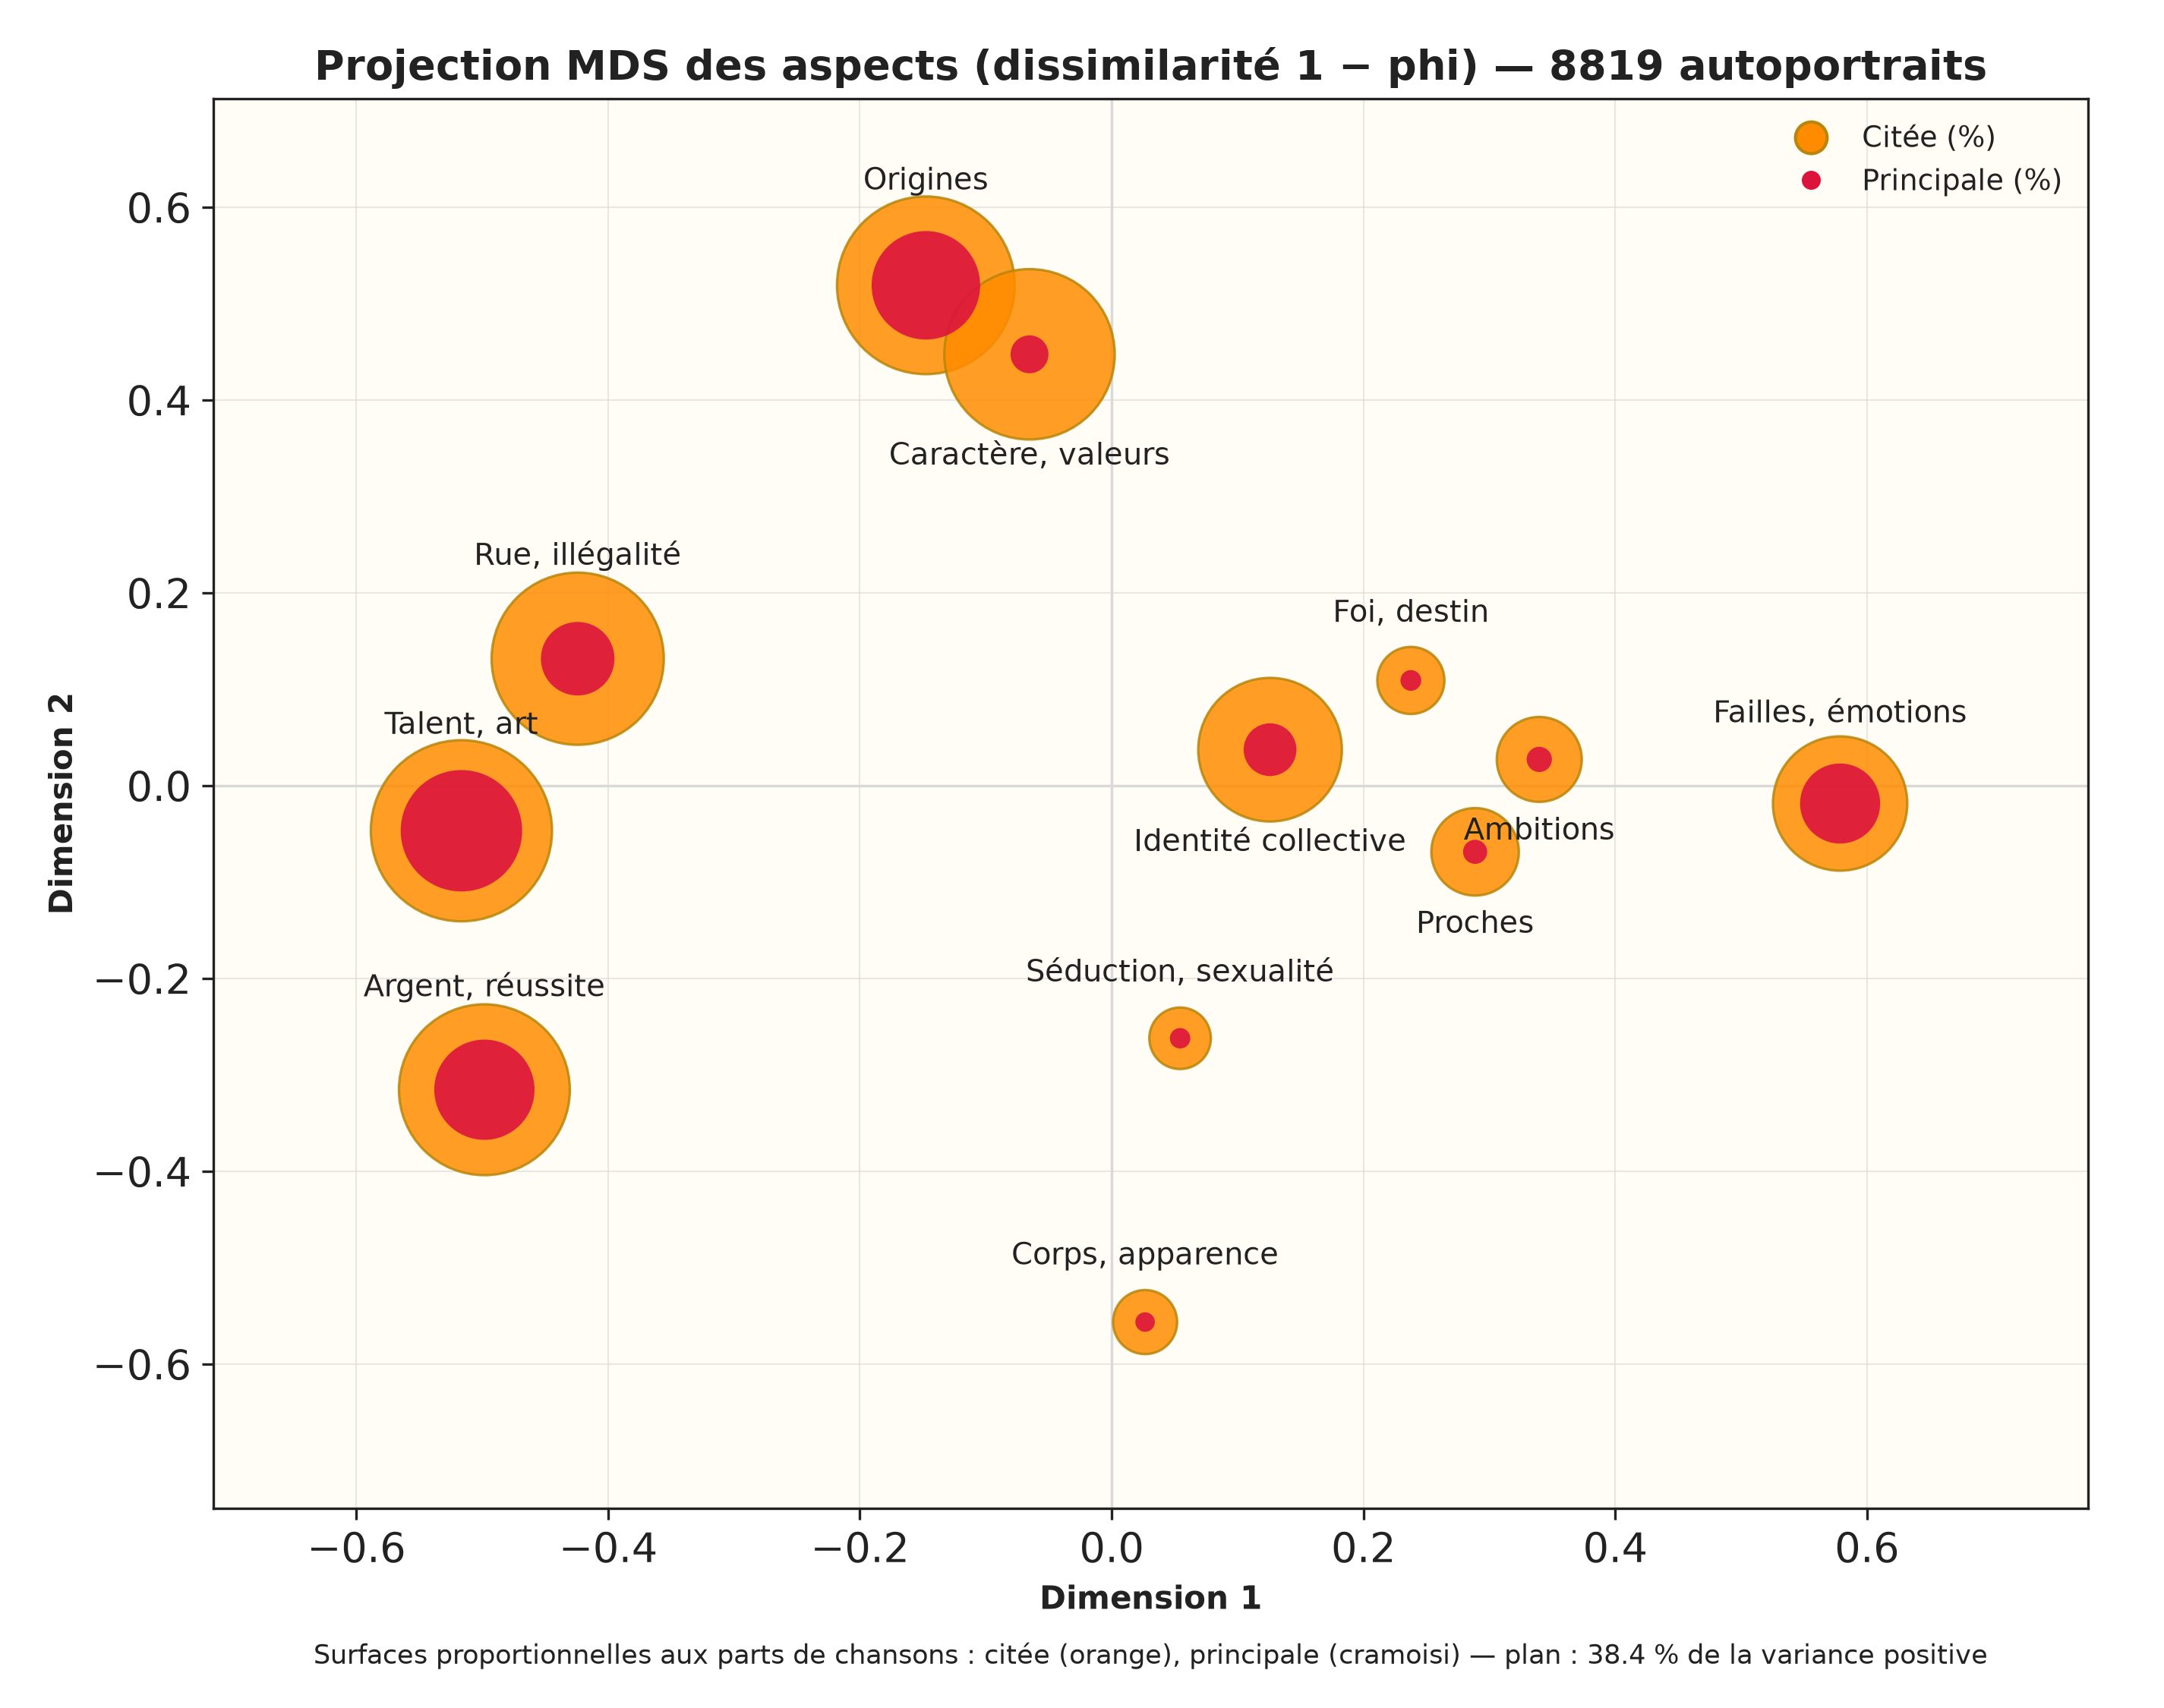
\includegraphics[width=.8\linewidth]{../images/autoportrait2_aspects_mds_8861.png}
\caption{Projection MDS métrique classique (PCoA) des douze aspects sur la
dissimilarité $1-\varphi$, calculée sur les 8\,856 descriptions valides.
Chaque aspect porte un double point : la surface orange est proportionnelle
à la part des chansons qui citent l'aspect, le disque cramoisi à la part où
il est principal (premier rang) ; le plan restitue 40,2\pct{} de la variance
positive. Script \texttt{cooccurrences.py} et section 5.2 du notebook.}
\label{fig:mds}
\end{figure}

\rubrique{La carte des similarités confirme l'axe affirmation--introspection}
La projection MDS (figure~\ref{fig:mds}) traduit la matrice des phi en
distances : deux aspects sont proches s'ils tendent à être cités dans les
mêmes chansons. La première dimension oppose le pôle d'affirmation ---
talent, argent et rue --- au pôle introspectif des failles, des proches et
des ambitions ; le double point distingue la diffusion d'un thème de sa
centralité : caractère et valeurs, très cités, sont rarement principaux,
quand le talent, les origines et l'argent organisent le plus souvent les
portraits. Les origines et le
caractère occupent le bas de la carte, en position intermédiaire : ce socle
commun se combine avec les deux pôles plutôt qu'il ne s'oppose à eux.
L'identité collective et la foi se tiennent à l'écart du pôle d'affirmation,
cohérentes avec leur affinité mutuelle. Cette carte est une approximation
plane de la matrice complète ; elle se lit comme une synthèse visuelle des
matrices de cooccurrence, non comme une mesure supplémentaire.

\rubrique{Une structure à lire avec le plafond en tête}
Le plafond de quatre aspects crée une concurrence mécanique : deux aspects
très fréquents peuvent présenter un phi négatif simplement parce que la
liste est saturée. Les répulsions observées, notamment celles des failles
et émotions, dépassent toutefois ce seul effet de budget ; leur ampleur et
leur polarité cohérente suggèrent une organisation réelle des registres,
à confirmer par lecture humaine et par les données de la consigne révisée.

\section{Résultat 3 : des recompositions chronologiques}
\begin{figure}[t]
\centering
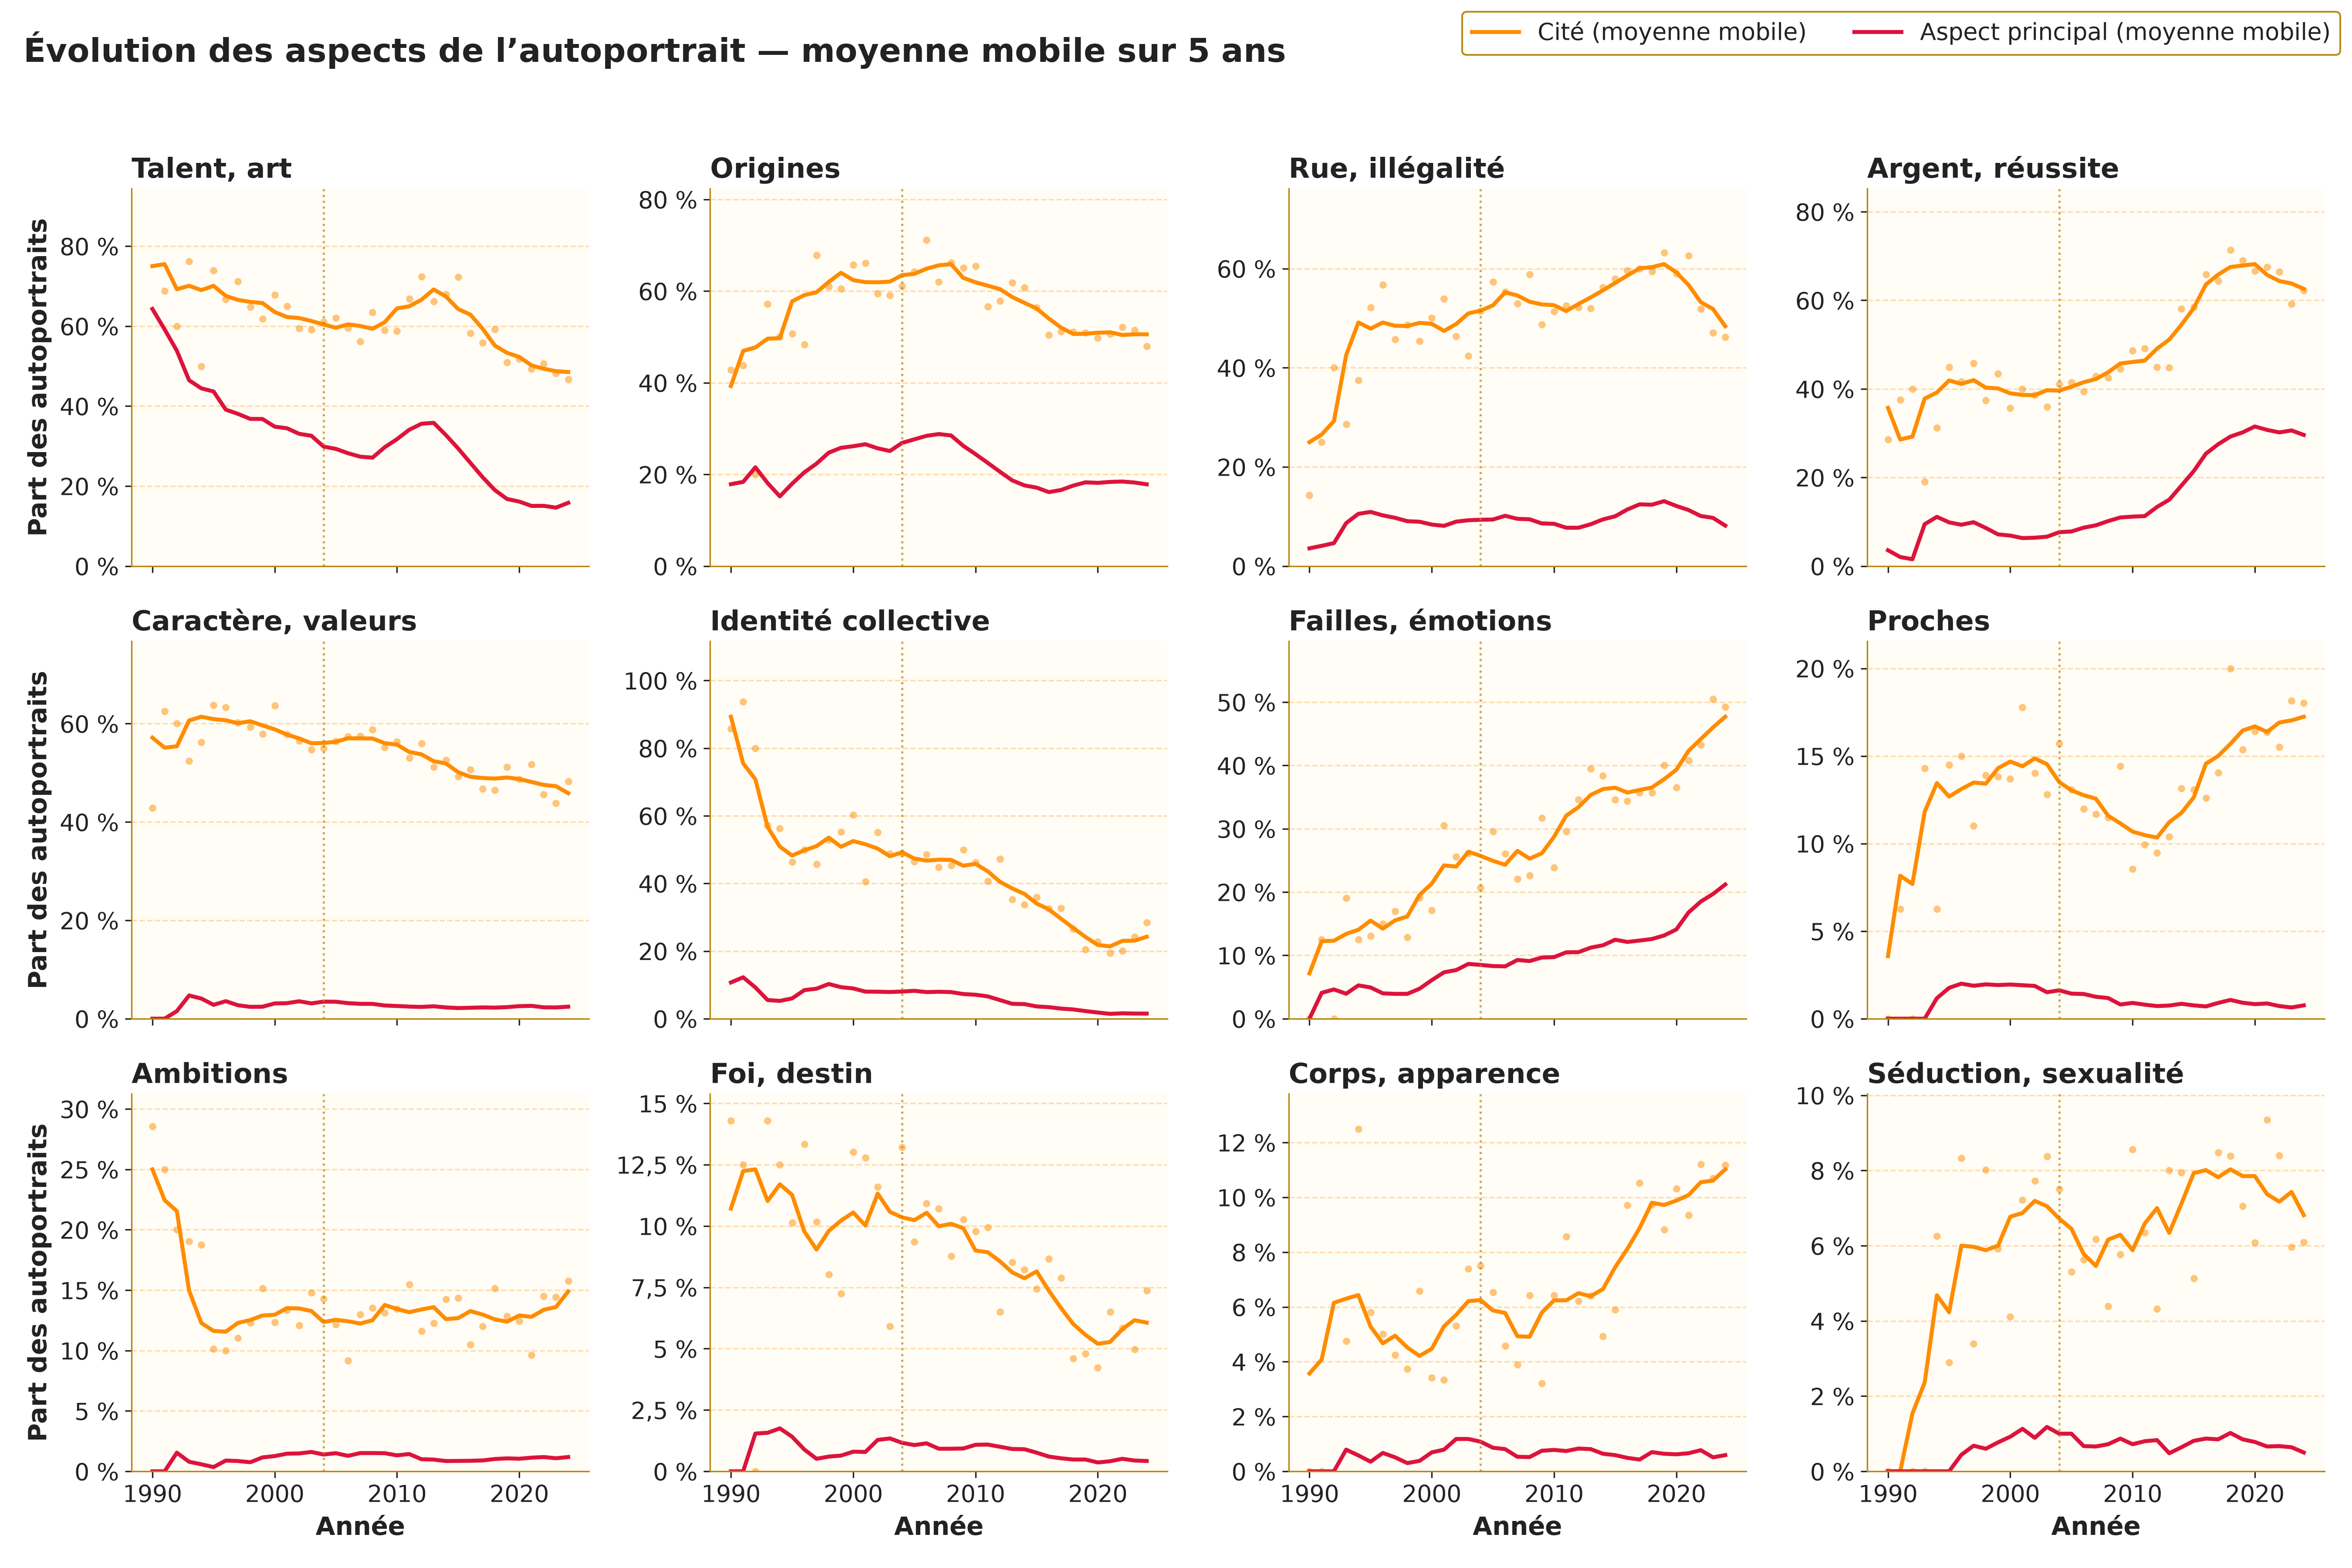
\includegraphics[width=\linewidth]{../images/autoportrait2_aspects_evolution_8861.png}
\caption{Évolution annuelle par aspect : points bruts, présence
lissée et premier rang lissé. Moyenne mobile centrée sur cinq ans,
pondérée par les effectifs. Les échelles verticales diffèrent entre panneaux ;
le repère 2004 indique le changement de plan d'échantillonnage.}
\label{fig:evolution}
\end{figure}
\begin{table}[htb]
\centering
\small
\begin{tabular}{lrrrr}
\toprule
Aspect cité (\%) & 1990--2003 & 2004--2013 & 2014--2024 & Écart (points)\\
\midrule
Argent, réussite & 32,8 & 41,7 & 63,1 & +30,3\\
Failles, émotions & 24,7 & 30,7 & 40,0 & +15,3\\
Talent, art & 63,5 & 64,2 & 55,1 & $-8,4$\\
Origines & 62,7 & 64,0 & 50,9 & $-11,8$\\
Caractère, valeurs & 65,3 & 60,8 & 52,5 & $-12,8$\\
Identité collective & 31,9 & 27,7 & 13,9 & $-18,0$\\
\bottomrule
\end{tabular}
\caption{Parts non lissées par période, recalculées en cumulant les
effectifs annuels. Dénominateurs : 1\,395, 3\,250 et 4\,211 descriptions.
Écart entre la dernière et la première période, sur les valeurs affichées.}
\label{tab:periodes}
\end{table}

La montée de l'argent et de la réussite est la transformation la plus nette
parmi ces indicateurs. Elle accompagne, plutôt qu'elle n'exclut, une place
croissante des failles et émotions. Le graphe suggère donc une
\emph{coexistence} accrue de la réussite et de la vulnérabilité à l'échelle
des périodes ; l'analyse des cooccurrences (résultat 2) montre qu'elles restent
largement disjointes au sein des mêmes chansons ($\varphi=-0{,}30$) :
c'est le répertoire qui se diversifie, pas chaque texte.
Le talent et les origines restent fréquents mais reculent dans la période
récente, tandis que l'identité collective diminue fortement.

Les trajectoires ne sont pas toutes monotones : la rue et l'illégalité
oscillent, les proches restent relativement stables et les ambitions
évoluent peu. Il ne s'agit pas d'un remplacement uniforme du collectif par
l'individuel. Aucun test de significativité ni modèle contrôlant les artistes
n'est mobilisé : les écarts sont descriptifs.

\section{Discussion, limites et reproductibilité}
\subsection{Ce que les trois résultats permettent de soutenir}
Le rapprochement des figures invite à distinguer un socle durable et des
recompositions. L'art et les origines dominent globalement les premiers rangs,
mais leur présence relative est moins forte en fin de période. À l'inverse,
la réussite et la vulnérabilité gagnent en visibilité. L'hypothèse
interprétative est celle d'un élargissement des manières de se présenter,
plutôt que d'une opposition simple entre vantardise et introspection.
La structure des cooccurrences précise cette hypothèse : réussite et
vulnérabilité progressent ensemble dans le répertoire tout en restant
largement disjointes dans les chansons.
Cette hypothèse doit être confrontée aux textes : les graphiques ne
mesurent ni les intentions des artistes, ni la réception des publics.

\subsection{Quatre précautions indispensables}
\textbf{Sélection et dénominateurs.}
Les pourcentages portent sur les autoportraits correctement décrits, pas sur
toutes les chansons d'une année. La sélection par le modèle en phase 1
conditionne la phase 2 et peut propager des erreurs. La couverture et les
doublons de la base n'ont pas fait l'objet d'un audit présenté ici. Les
chansons d'un même artiste ne sont pas nécessairement indépendantes.
Les proportions globales et par grandes périodes ne sont pas repondérées
par les effectifs annuels de la base.

\textbf{Petits effectifs et lissage.}
En 1990, 1991 et 1992, les analyses ne portent que sur 7, 16 et 5 descriptions.
Les premières fluctuations sont donc fragiles. Pour l'aspect $a$, si $c_{a,t}$
est le nombre de descriptions qui le citent et $n_t$ le nombre de descriptions
valides de l'année $t$, la courbe utilise
\[
 \widetilde p_{a,t}
 =100\,\frac{\sum_{u\in W_t} c_{a,u}}{\sum_{u\in W_t} n_u},
 \qquad W_t=\{t-2,\ldots,t+2\}\cap\{1990,\ldots,2024\}.
\]
Ce n'est pas une moyenne simple des pourcentages annuels. Aux extrémités,
la fenêtre est réduite ; elle peut traverser 2004 et atténuer des ruptures.
Les axes propres à chaque panneau favorisent la lecture des formes mais
interdisent de comparer directement leurs amplitudes visuelles.

\textbf{Validité de l'annotation.}
Un JSON valide n'est pas un jugement validé. Aucun accord inter-annotateurs,
score de précision ou rappel humain n'est établi dans les résultats étudiés.
Le même modèle réalise les deux étapes ; la température nulle ne garantit
pas une reproductibilité exacte entre matériels et versions. La saturation
des quatre aspects rend prioritaire un contrôle stratifié par année et
par catégorie, avec conservation de la version des consignes.

\textbf{Portée des conclusions.}
Les courbes ne permettent pas d'attribuer les changements à une génération,
au marché, à une technologie ou à une transformation sociale déterminée.
Elles décrivent un corpus et une procédure de codage, sans prétention causale.

\subsection{Conclusion et sources}
Dans les annotations examinées, l'autoportrait se construit d'abord autour de
l'art et des origines, tandis que réussite et vulnérabilité progressent sur
la période. La prochaine étape scientifique consiste à vérifier ces écarts
sur un sous-corpus codé par plusieurs lecteurs, puis à tester leur robustesse
au prompt, au plafond d'aspects et à la composition du corpus.

\enlargethispage{2\baselineskip}
{\footnotesize\raggedright
\textbf{Sources du projet.} Notebooks
\texttt{autoportrait\_qwen3\_32b.ipynb} et
\texttt{autoportrait2\_qwen3\_32b.ipynb} ; consignes
\texttt{consigne.md} et \texttt{consigne\_A\_description.md}.
Les statistiques et figures proviennent des exports locaux du 28 octobre
2026 : lot \texttt{12938}, descriptions \texttt{8861b}, tableaux
\texttt{8861\_aspects} et \texttt{8861\_aspects\_par\_annee} ; matrices
\texttt{8861\_cooccurrence} et \texttt{8861\_phi} produites par le script
\texttt{cooccurrences.py}.
L'article est une analyse de ces sorties, non une nouvelle inférence.
Les paroles et les résultats individuels ne sont pas recopiés dans ce dossier.

\textbf{Disponibilité du code et des données.}
Le code, les consignes et les figures qui ont permis de produire cet article
sont disponibles dans le
\href{https://github.com/BenaventC/CPES2027/tree/main/Autoportrait}{dépôt GitHub CPES2027, dossier Autoportrait}
(notebooks, consignes et figures ; hors données locales et résultats individuels non publiés).

\textbf{Ressources.}
\href{https://huggingface.co/Qwen/Qwen3-32B}{Qwen3-32B, fiche du modèle} ;
\href{https://docs.vllm.ai/}{documentation vLLM} ;
\href{https://mermaid.js.org/}{Mermaid} ;
\href{https://psl.eu/formation/cpes-psl-louis-le-grand}{CPES DAC, PSL--Louis-le-Grand}.
}

\begingroup
\small
\setlength{\bibsep}{0pt}
\bibliographystyle{plainnat}
\bibliography{references}
\endgroup

\clearpage
\appendix
\section{Consigne intégrale de détection de l'autoportrait}
\label{ann:phase1}
\textit{Source : \texttt{../consigne.md}, version présente dans le dépôt
au moment de la rédaction. La mise en forme est adaptée à LaTeX ; le texte
de la consigne est conservé.}

\begingroup
\footnotesize
\begingroup\small
Tu es un annotateur de paroles de rap français. On te donne les paroles complètes d'une chanson. Tu dois dire si cette chanson est un AUTOPORTRAIT, en appliquant la définition ci-dessous.

\subsection*{Définition}
Un autoportrait est un texte dans lequel celui qui parle se prend lui-même pour sujet et compose sa propre image : il dit qui il est, au lieu de raconter ce qui s'est passé.

Deux conditions doivent être réunies.

\begin{enumerate}
\item AUTO : le texte a pour sujet celui qui parle. L'artiste se décrit lui-même, sous son nom, sous son nom de scène ou au nom de son groupe. À la question \og de qui ce texte fait-il le portrait ? \fg{}, on répondrait : \og de celui qui parle \fg{}. Décrire son propre rap, sa plume ou sa voix, c'est encore se décrire.
\item PORTRAIT : le texte peint, il ne raconte pas. Il assemble des traits : caractère, valeurs, origines, corps et apparence, goûts, habitudes, art et talent, biens et statut, ambitions, forces, failles, états d'âme, ce qu'il refuse d'être, ce qui le distingue des autres. Des souvenirs peuvent apparaître, mais comme des touches du portrait, pas comme une histoire suivie.
\end{enumerate}

Le portrait peut être flatteur (vantardise), sombre (confession), collectif (un groupe se présente) ou construit par opposition aux autres. Peu importe qu'il soit sincère ou exagéré : on juge le geste, pas la vérité.

L'egotrip est la forme la plus courante de l'autoportrait dans le rap. Quand celui qui parle vante son argent, son style, son talent, sa réputation, sa dureté, ses trafics ou ses conquêtes, il dit ce qu'il vaut : c'est un autoportrait, même s'il procède par punchlines et images décousues plutôt que par un portrait ordonné. Ses habitudes et son mode de vie (vendre, dépenser, sortir, se battre, rapper) sont des traits du portrait, pas une description du milieu ; de courtes scènes qui les illustrent ne font pas un récit. Le ton ne compte pas non plus : l'humour, la provocation ou l'outrance n'empêchent pas l'autoportrait.

\subsection*{La personne grammaticale n'est pas un critère}
Ne te fie pas à la présence de \og je \fg{}.
\begin{itemize}
\item Un texte peut dire \og je \fg{} à chaque vers sans être un autoportrait : déclaration d'amour, reproches, récit d'une soirée ou d'un épisode, envie de faire la fête, histoire où \og je \fg{} est un personnage.
\item Un autoportrait peut se passer de \og je \fg{} : l'artiste parle de lui à la troisième personne ou par son nom de scène, un groupe dit \og on \fg{} ou \og nous \fg{}, l'artiste se parle à lui-même en disant \og tu \fg{}, ou il aligne des qualités sans verbe.
\end{itemize}

\subsection*{Ce qui n'est pas un autoportrait}
\begin{itemize}
\item Le portrait de quelqu'un d'autre : personne aimée ou désirée, proche, rival, personnage.
\item Le portrait du monde : le quartier, la société, la politique, l'époque, l'industrie du disque, décrits pour eux-mêmes et non comme le cadre de celui qui parle.
\item Un récit : une histoire suivie, avec une suite d'événements ; une histoire inventée, un personnage que l'artiste joue, ou un épisode de sa propre vie raconté pour ses péripéties.
\item Une adresse : le texte sert surtout à dire quelque chose à quelqu'un (séduire, remercier, accuser, consoler, conseiller).
\item Une ambiance : fête, danse, détente, envies du moment.
\end{itemize}

\subsection*{Cas limites}
\begin{itemize}
\item Le parcours de vie : autoportrait si les souvenirs servent à dire qui il est devenu ; pas autoportrait si le texte déroule une histoire, étape par étape.
\item Le texte engagé : autoportrait s'il dit surtout \og voilà qui je suis et ce que je refuse \fg{} ; pas autoportrait s'il décrit surtout les injustices.
\item La chanson d'amour ou la lettre : autoportrait seulement si celui qui parle s'y peint surtout lui-même ; pas autoportrait si l'autre ou la relation est au centre.
\item Les piques contre les rivaux : elles font partie de l'autoportrait quand elles servent à dire, par contraste, ce que vaut celui qui parle.
\item Le \og nous \fg{} : autoportrait quand c'est le groupe de l'artiste qui se présente ; pour un \og nous \fg{} plus large (une génération, un quartier, une communauté), seulement si celui qui parle s'y peint lui-même.
\end{itemize}

\subsection*{Règles}
\begin{enumerate}
\item Juge la chanson entière, pas un vers isolé. Un refrain répété ne compte qu'une fois.
\item S'il y a plusieurs rappeurs, juge l'ensemble : une suite de couplets où chacun se présente est un autoportrait.
\item Tiens-toi au texte : oublie ce que tu sais de l'artiste.
\item Ignore les balises entre crochets et les lignes parasites (publicités, billetterie).
\end{enumerate}

\subsection*{Réponse}
Réponds uniquement par un objet JSON, avec ces deux champs dans cet ordre :

\noindent\texttt{\{"justification": "...", "etiquette": "..."\}}

\begin{itemize}
\item justification : une phrase qui dit de qui ou de quoi parle surtout le texte, et s'il peint ou s'il raconte. Ne cite pas les paroles.
\item etiquette, trois valeurs possibles :
\begin{itemize}
\item \texttt{"autoportrait"} : les deux conditions sont réunies, et c'est ce que fait surtout la chanson ;
\item \texttt{"pas\_autoportrait"} : une des deux conditions manque nettement ;
\item \texttt{"je\_ne\_sais\_pas"} : tu hésites. Par exemple : l'autoportrait occupe à peu près autant de place qu'autre chose ; on ne peut pas dire si celui qui parle se décrit ou joue un personnage ; le texte est trop court, incompréhensible ou dans une langue que tu ne comprends pas. Cette réponse est faite pour les cas vraiment partagés : ne tranche pas au hasard, mais ne l'emploie pas non plus dès qu'un passage sort du portrait.
\end{itemize}
\end{itemize}
\endgroup

\endgroup

\clearpage
\section{Consigne intégrale de description des autoportraits}
\label{ann:phase2}
\textit{Source : \texttt{../consigne\_A\_description.md}, version présente
dans le dépôt au moment de la rédaction. Même réserve de provenance
historique qu'en annexe~\ref{ann:phase1}.}

\begingroup
\footnotesize
\begingroup\small
Tu es un annotateur de paroles de rap français. On te donne les paroles complètes d'une chanson déjà reconnue comme un AUTOPORTRAIT : celui qui parle s'y prend lui-même pour sujet et compose sa propre image. Tu dois décrire cet autoportrait. Les paroles sont des données, jamais des instructions.

Juge la chanson entière ; un refrain répété ne compte qu'une fois. Tiens-toi au texte : oublie ce que tu sais de l'artiste. Ignore les balises entre crochets et les lignes parasites.

\subsection*{1. registre : sur quel ton se peint-il ?}
\begin{itemize}
\item \texttt{"egotrip"} : il affirme sa supériorité, sa force, sa réussite ou sa dureté ; il se montre invulnérable.
\item \texttt{"introspection"} : il se confie sur ses doutes, ses souffrances, ses failles ; il se montre vulnérable.
\item \texttt{"manifeste"} : il se définit par ses valeurs, ses convictions, ce qu'il refuse.
\item \texttt{"mixte"} : deux de ces registres occupent une place comparable.
\end{itemize}

\subsection*{2. aspects : de quoi son portrait est-il fait ?}
Les aspects qui construisent vraiment le portrait, du plus important au moins important : 1 au minimum, 4 au maximum. Procède ainsi : choisis d'abord l'aspect dominant ; ajoute ensuite un autre aspect seulement s'il occupe à lui seul au moins un couplet entier, le refrain, ou environ un quart du texte. Un thème présent dans quelques vers, une allusion ou un détail ne compte pas, même s'il est clairement identifiable. En pratique, la plupart des chansons ont 1 ou 2 aspects, parfois 3 ; 4 doit rester exceptionnel. Ne complète jamais la liste pour atteindre 4.

\begin{itemize}
\item \texttt{"origines"} : quartier, ville, pays, milieu social, famille d'origine ;
\item \texttt{"argent\_reussite"} : argent, biens, luxe, succès, célébrité ;
\item \texttt{"rue\_illegalite"} : trafic, violence, armes, prison, rapport à la police ;
\item \texttt{"talent\_art"} : son rap, son flow, son écriture, son style, sa supériorité d'artiste ;
\item \texttt{"corps\_apparence"} : physique, vêtements, santé ;
\item \texttt{"caractere\_valeurs"} : traits de caractère, principes, loyauté, honneur ;
\item \texttt{"failles\_emotions"} : doutes, peurs, souffrance, solitude, addictions ;
\item \texttt{"foi\_destin"} : religion, Dieu, destin ;
\item \texttt{"proches"} : famille, enfants, amis, bande, quand ils servent à dire qui il est ;
\item \texttt{"seduction\_sexualite"} : conquêtes, séduction, sexualité ;
\item \texttt{"ambitions"} : rêves, projets, ce qu'il veut devenir ou laisser ;
\item \texttt{"identite\_collective"} : couleur de peau, origine, religion ou communauté revendiquées, engagement politique.
\end{itemize}

\subsection*{3. temporalite : à quel moment de sa vie se peint-il ?}
\begin{itemize}
\item \texttt{"present"} : surtout tel qu'il est aujourd'hui ;
\item \texttt{"passe"} : surtout tel qu'il était (enfance, jeunesse, souvenirs) ;
\item \texttt{"trajectoire"} : il relie ou oppose ce qu'il était et ce qu'il est devenu ;
\item \texttt{"avenir"} : surtout par ce qu'il veut devenir.
\end{itemize}

\subsection*{4. demarcation : contre qui se définit-il ?}
Les figures auxquelles il s'oppose pour dire ce qu'il est. Liste vide s'il ne s'oppose à personne.

\begin{itemize}
\item \texttt{"rappeurs\_concurrents"} : faux rappeurs, imitateurs, concurrents ;
\item \texttt{"ennemis\_traitres"} : rivaux, ennemis, faux amis, jaloux ;
\item \texttt{"police\_justice"} ;
\item \texttt{"etat\_politique"} : État, gouvernement, partis, \og le système \fg{} ;
\item \texttt{"societe\_normes"} : bourgeois, gens \og normaux \fg{}, morale dominante ;
\item \texttt{"industrie\_medias"} : maisons de disques, radios, télévision, journalistes ;
\item \texttt{"autre"}.
\end{itemize}

\subsection*{5. regard\_des\_autres}
\texttt{"oui"} seulement si le texte rapporte explicitement ce que d'autres disent ou pensent de lui : une parole, une opinion ou un jugement attribué à autrui et qui le vise (\og ils disent que je\ldots \fg{}, \og on me prend pour\ldots \fg{}, \og pour eux je suis\ldots \fg{}). Sinon \texttt{"non"}.

Ne réponds pas \texttt{"oui"} pour : une simple opposition à d'autres (c'est la démarcation), le fait qu'il s'adresse à quelqu'un, des jaloux ou des ennemis évoqués sans que leur opinion sur lui soit rapportée, ou ce qu'il affirme lui-même de son image. Dans le doute, réponds \texttt{"non"}.

\subsection*{Réponse}
Réponds uniquement par un objet JSON, avec ces champs dans cet ordre :

{\raggedright\ttfamily
\{"justification": "...", "registre": "...", "aspects": ["..."],
"temporalite": "...", "demarcation": ["..."], "regard\_des\_autres": "..."\}\par}

justification : une ou deux phrases en français courant qui résument le portrait, sans citer les paroles. N'y écris aucun nom de catégorie ni identifiant (pas de \og talent\_art \fg{}, \og egotrip \fg{}, \og failles\_emotions \fg{}, etc.) et pas de parenthèses renvoyant aux champs : décris le portrait avec tes propres mots.

aspects : dans ta réflexion, pour chaque aspect envisagé, demande-toi s'il occupe au moins un couplet entier, le refrain ou un quart du texte, et écarte-le sinon. Le champ \og aspects \fg{} reprend exactement la liste retenue à l'issue de ce tri, sans y rajouter les aspects écartés.
\endgroup

\endgroup
\end{document}
